% Mestre em LaTeX - v0.2
% Copyleft 2008-2011 Bruno C. Vellutini - http://organelas.com/
%
% Permission is hereby granted, free of charge, to any person obtaining a copy
% of this software and associated documentation files (the "Software"), to deal
% in the Software without restriction, including without limitation the rights
% to use, copy, modify, merge, publish, distribute, sublicense, and/or sell
% copies of the Software, and to permit persons to whom the Software is
% furnished to do so, subject to the following conditions:
%
% THE SOFTWARE IS PROVIDED "AS IS", WITHOUT WARRANTY OF ANY KIND, EXPRESS OR
% IMPLIED, INCLUDING BUT NOT LIMITED TO THE WARRANTIES OF MERCHANTABILITY,
% FITNESS FOR A PARTICULAR PURPOSE AND NONINFRINGEMENT. IN NO EVENT SHALL THE
% AUTHORS OR COPYRIGHT HOLDERS BE LIABLE FOR ANY CLAIM, DAMAGES OR OTHER
% LIABILITY, WHETHER IN AN ACTION OF CONTRACT, TORT OR OTHERWISE, ARISING FROM,
% OUT OF OR IN CONNECTION WITH THE SOFTWARE OR THE USE OR OTHER DEALINGS IN
% THE SOFTWARE.
%
% Ou seja, utilize e modifique os arquivos como desejar.
% 
% Para mais informações visite http://code.google.com/p/mestre-em-latex/

% Classe do documento
\documentclass[twoside,a4paper,11pt]{report}

% Pacotes e comandos customizados
%%% Pacotes utilizados %%%

%% Codificação e formatação básica do LaTeX
% Suporte para português (hifenação e caracteres especiais)
\usepackage[english,brazilian]{babel}

% Codificação do arquivo
\usepackage[utf8]{inputenc}

% Mapear caracteres especiais no PDF
\usepackage{cmap}

% Codificação da fonte
\usepackage[T1]{fontenc}

%% Microtipografia
% Utiliza recursos como espaçamento entre letras e entre linhas
\usepackage{microtype}
% Habilita protrusão e expansão, ignorando
% compatibilidade (ver documentação do pacote)
\microtypesetup{activate={true,nocompatibility}}
% factor=1100 aumenta a protrusão (default 1000)
% stretch=10 diminui o valor máximo de expansão (default 20)
% shrink=10 diminui o valor máximo de encolhimento (default 20)
\microtypesetup{factor=1100, stretch=10, shrink=10}
% Tracking, espaçamento entre palavras, kerning
\microtypesetup{tracking=true, spacing=true, kerning=true}
% Remover tracking para Small Caps
\SetTracking{encoding={T1}, shape=sc}{0}
% Remove ligaduras para o 'f'. Se necessário, adicionar letras
% separadas por vírgulas
\DisableLigatures[f]{encoding={T1}}
% Documento em versão "final", suporte para outros idiomas
\microtypesetup{final, babel}

% Essencial para colocar funções e outros símbolos matemáticos
\usepackage{amsmath,amssymb,amsfonts,textcomp}

%% Layout
% Customização do layout da página, margens espelhadas
\usepackage[twoside]{geometry}
% Aumenta as margens internas para espiral
\geometry{bindingoffset=10pt}
% Só pra ajustar o layout
\setlength{\marginparwidth}{90pt}
%\usepackage{layout}

% Para definir espaçamento entre as linhas
\usepackage{setspace}

% Espaçamento do texto para o frame
\setlength{\fboxsep}{1em}

% Faz com que as margens tenham o mesmo tamanho horizontalmente
%\geometry{hcentering}

%% Elementos Gráficos
% Para incluir figuras (pacote extendido)
\usepackage[]{graphicx}

\graphicspath{{figuras/}}

%% Suporte a cores
\usepackage{color}
% Os argumentos declaram nomes novos, como Cyan e Crimson
% (ver documentação do pacote).
\usepackage[usenames,dvipsnames,svgnames]{xcolor}

% Criar figura dividida em subfiguras
\usepackage{subfig}
%\captionsetup[subfigure]{style=default, margin=0pt, parskip=0pt, hangindent=0pt, indention=0pt, singlelinecheck=true, labelformat=parens, labelsep=space}

% Caso queira guardar as figuras em uma pasta separada
% (descomente e) defina o caminho para o diretório:
%\graphicspath{{./figuras/}}

% Customizar as legendas de figuras e tabelas
\usepackage{caption}

% Criar ambientes com 2 ou mais colunas
\usepackage{multicol}

% Ative o comando abaixo se quiser colocar figuras de fundo (e.g., capa)
%\usepackage{wallpaper}
% Exemplo para inserir a figura na capa está no arquivo pre.tex (linha 7)
% Ajuste da posição da figura no eixo Y
%\addtolength{\wpYoffset}{-140pt}
% Ajuste da posição da figura no eixo X
%\addtolength{\wpXoffset}{36pt}

%% Tabelas
% Elementos extras para formatação de tabelas
\usepackage{array}

% Tabelas com qualidade de publicação
\usepackage{booktabs}

% Para criar tabelas maiores que uma página
\usepackage{longtable}

% adicionar tabelas e figuras como landscape
\usepackage{lscape}

%% Lista de Abreviações
% Cria lista de abreviações
\usepackage[notintoc,portuguese]{nomencl}
\makenomenclature

%% Notas de rodapé
% Lidar com notas de rodapé em diversas situações
\usepackage{footnote}

% Notas criadas nas tabelas ficam no fim das tabelas
\makesavenoteenv{tabular}

% Conta o número de páginas
\usepackage{lastpage}

%% Referências bibliográficas e afins
% Formatar as citações no texto e a lista de referências
\usepackage{natbib}

% Adicionar bibliografia, índice e conteúdo na Tabela de conteúdo
% Não inclui lista de tabelas e figuras no índice
\usepackage[nottoc,notlof,notlot]{tocbibind}

%% Pontuação e unidades
% Posicionar inteligentemente a vírgula como separador decimal
\usepackage{icomma}

% Formatar as unidades com as distâncias corretas
\usepackage[tight]{units}

%% Cabeçalho e rodapé
% Controlar os cabeçalhos e rodapés
\usepackage{fancyhdr}
% Usar os estilos do pacote fancyhdr
\pagestyle{fancy}
\fancypagestyle{plain}{\fancyhf{}}
% Limpar os campos do cabeçalho atual
\fancyhead{}
% Número da página do lado esquerdo [L] nas páginas ímpares [O] e do lado direito [R] nas páginas pares [E]
\fancyhead[LO,RE]{\thepage}
% Nome da seção do lado direito em páginas ímpares
\fancyhead[RO]{\nouppercase{\rightmark}}
% Nome do capítulo do lado esquerdo em páginas pares
\fancyhead[LE]{\nouppercase{\leftmark}}
% Limpar os campos do rodapé
\fancyfoot{}
% Omitir linha de separação entre cabeçalho e conteúdo
\renewcommand{\headrulewidth}{0pt}
% Omitir linha de separação entre rodapé e conteúdo
\renewcommand{\footrulewidth}{0pt}
% Altura do cabeçalho
\headheight 13.6pt

% Dados do projeto
\newcommand{\nomedoaluno}{Nome Completo do Aluno}
\newcommand{\titulo}{Título original do projeto}

%% Links dinâmicos
% Suporte para hipertexto, links para referências e figuras
\usepackage{hyperref}
% Configurações dos links e metatags do PDF a ser gerado
\hypersetup{colorlinks=true, linkcolor=blue, citecolor=blue, filecolor=blue, urlcolor=green,
            pdfauthor={\nomedoaluno},
            pdftitle={\titulo},
            pdfsubject={Assunto do Projeto},
            pdfkeywords={palavra-chave, palavra-chave, palavra-chave},
            pdfproducer={LaTeX},
            pdfcreator={pdfTeX}}

%% Inserir comentários no texto
% Marcar mudanças e fazer comentários
%\usepackage[margins]{trackchanges}
% Iniciais do autor
%\renewcommand{\initialsTwo}{bcv}
% Notas na margem interna
%\reversemarginpar

%% Comandos customizados

% Espécie e abreviação
\newcommand{\subde}{\emph{Clypeaster subdepressus}}
\newcommand{\subsus}{\emph{C.~subdepressus}}

%% Pacotes não implementados
% Para não sobrar espaços em branco estranhos
%\widowpenalty=1000
%\clubpenalty=1000


\usepackage{ucs}


%\theoremstyle{definition}
\newtheorem{defi}{Definição}
\newtheorem{exem}{Exemplo}
\newtheorem{teo}{Teorema}
\newcommand{\setof}[1]{\ensuremath{\left \{ #1 \right \}}}
\newcommand{\tuple}[1]{\ensuremath{\left \langle #1 \right \rangle }}

%% pacotes para o cronograma
\usepackage{colortbl}
\usepackage{booktabs}
\newcommand{\mc}[3]{\multicolumn{#1}{#2}{#3}}
\definecolor{tcA}{gray}{0}

% Início do texto
\begin{document}

% Limpa cabeçalhos.
% (solução para lidar com a númeração das páginas pré-textuais).
\pagestyle{empty}

%% Capa
\begin{titlepage}

% Se quiser uma figura de fundo na capa ative o pacote wallpaper
% e descomente a linha abaixo.
% \ThisCenterWallPaper{0.8}{nomedafigura}

\begin{center}
{\LARGE Daniel Nascimento Teixeira}
\par
\vspace{200pt}
{\Huge Uma Técnica de Particionamento Aprori para Malhas Triangulares utilizando Quadtree}
\par
\vfill
\textbf{{\large Fortaleza}\\
{\large \the\year}}
\end{center}
\end{titlepage}

% Faz com que a página seguinte sempre seja ímpar (insere pg em branco)
\cleardoublepage

% Numeração em elementos pré-textuais é opcional (ativada por padrão).
% Para desativá-la comente a linha abaixo.
\pagestyle{fancy}

% Números das páginas em algarismos romanos
\pagenumbering{roman}

%% Página de Rosto

% Numeração não deve aparecer na página de rosto.
\thispagestyle{empty}

\begin{center}
{\LARGE Daniel Nascimento Teixeira}
\par
\vspace{200pt}
{\Huge Uma Técnica de Particionamento Aprori para Malhas Triangulares utilizando Quadtree}
\end{center}
\par
\vspace{90pt}
\hspace*{175pt}\parbox{7.6cm}{{\large Dissertação apresentada ao Departamento de Computação da Universidade Federal do Ceará, para a obtenção de Título de Mestre}}

\par
\vspace{1em}
\hspace*{175pt}\parbox{7.6cm}{{\large Orientador: Joaquim Bento}}

\par
\vfill
\begin{center}
\textbf{{\large Fortaleza}\\
{\large \the\year}}
\end{center}

\newpage

% Ficha Catalográfica
\hspace{8em}\fbox{\begin{minipage}{10cm}
Aluno, Daniel Nascimento Teixeira.

\hspace{2em}Uma Técnica de Particionamento Aprori para Malhas Triangulares utilizando Quadtree

\hspace{2em}\pageref{LastPage} páginas

\hspace{2em}Dissertação (Mestrado) - Universidade Federal do Ceará. Departamento de Computação.

\begin{enumerate}
\item Malha triangular
\item Subdivisão de domínio
\item Quadtree
\end{enumerate}
I. Universidade Federal do Ceará. Departamento de Computação.

\end{minipage}}
\par
\vspace{2em}
\begin{center}
{\LARGE\textbf{Comissão Julgadora:}}

\par
\vspace{10em}
\begin{tabular*}{\textwidth}{@{\extracolsep{\fill}}l l}
\rule{16em}{1px} 	& \rule{16em}{1px} \\
Prof. Dr. 		& Prof. Dr. \\
Nome			& Nome
\end{tabular*}

\par
\vspace{10em}

\parbox{16em}{\rule{16em}{1px} \\
Prof. Dr. \\
Nome do Orientador}
\end{center}

\newpage

% Epígrafe
\vspace*{0.4\textheight}
\noindent{\LARGE\textbf{Epígrafe}}
% Tudo que você escreve no verbatim é renderizado literalmente (comandos não são interpretados e os espaços são respeitados)
\begin{verbatim}
Aprendi através da experiência amarga a suprema lição: 
controlar minha ira e torná-la como o calor que é convertido em energia. 
Nossa ira controlada pode ser convertida numa força capaz de mover o mundo.
\end{verbatim}
\begin{flushright}
Mahatma Gandhi
\end{flushright}

\newpage

% Agradecimentos

% Espaçamento duplo
\doublespacing

\noindent{\LARGE\textbf{Agradecimentos}}

Agradeço ao meu orientador, ao meu co-orientador, aos meus colaboradores, aos técnicos, à seção administrativa, à fundação que liberou verba para minhas pesquisas, aos meus amigos e à minha família.

\newpage

\vspace*{10pt}
% Abstract
\begin{center}
  \emph{\begin{large}Resumo\end{large}}\label{resumo}
\vspace{2pt}
\end{center}
% Pode parecer estranho, mas colocar uma frase por linha ajuda a organizar e reescrever o texto quando necessário.
% Além disso, ajuda se você estiver comparando versões diferentes do mesmo texto.
% Para separar parágrafos utilize uma linha em branco.
\noindent
Este trabalho descreve uma técnica de geração de malhas bidimensionais triangulares usando computadores paralelos com memória distribuída, baseado em um modelo de paralelismo mestre/escravos. Esta técnica utiliza uma \textit{quadtree} grosseira para decompor o domínio e um processo de avanço de fronteira serial para gerar a malha em cada subdomínio simultaneamente. Uma \textit{quadtree} fina é empregada neste trabalho para ajudar a estimar a carga de processamento associado a cada subdomínio. O nível de refinamento da \textit{quadtree} fina é usado para orientar a criação das arestas que são definidas pela discretização das células internas da \textit{quadtree} dos subdomínios. É mostrado que a técnica de estimativa de carga produz resultados que representam com precisão o número de elementos a serem gerados em cada subdomínio, levando a previsão de tempo de execução adequada e com um algoritmo bem balanceado. Quando comparado com o seu homólogo serial, a técnica em paralelo é muito mais rápida e muitas vezes apresenta um desempenho super-
linear. As malhas geradas com a técnica em paralelo têm a mesma qualidade como as geradas serialmente, dentro de limites aceitáveis​​. 
\par
\vspace{1em}
\noindent\textbf{Palavras-chave:} Malha triangular, Subdivisão de domínio, Quadtree
\newpage

% Criei a página do abstract na mão, por isso tem bem mais comandos do que o resumo acima, apesar de serem idênticas.
\vspace*{10pt}
% Abstract
\begin{center}
  \emph{\begin{large}Abstract\end{large}}\label{abstract}
\vspace{2pt}
\end{center}

% Selecionar a linguagem acerta os padrões de hifenação diferentes entre inglês e português.
\selectlanguage{english}
\noindent
This work describes a technique for generating two-dimensional triangular meshes using parallel computers with distributed memory, based on a master/slaves parallelism model. This technique uses a coarse quadtree to decompose the domain and a serial advancing front procedure to generate the mesh in each subdomain concurrently. A finer quadtree is employed in this work to help estimate the processing load associated with each subdomain. The level of refinement of this finer quadtree is used to guide the creation of the edges that define the quadtree's inter-cell discretization of the subdomains. It is shown that the load estimation technique produces results that accurately represent the number of elements to be generated in each subdomain, leading to proper runtime prediction and to a well-balanced algorithm. When compared with its serial counterpart, the parallel technique is much faster and often presents a super-linear performance. The meshes generated with the parallel technique have the same quality as 
those generated serially, within acceptable limits.
\par
\vspace{1em}
\noindent\textbf{Keywords:} Triangular mesh, Domain subdivision, Quadtree

% Voltando ao português...
\selectlanguage{brazilian}

\newpage

% Desabilitar protrusão para listas e índice
\microtypesetup{protrusion=false}

% Lista de figuras
\listoffigures

% Lista de tabelas
\listoftables

% Abreviações
% Para imprimir as abreviações siga as instruções em 
% http://code.google.com/p/mestre-em-latex/wiki/ListaDeAbreviaturas
%\printnomenclature

% Índice
\tableofcontents

% Re-habilita protrusão novamente
\microtypesetup{protrusion=true}
   % Capa, prefácio e afins
% Faz com que o ínicio do capítulo sempre seja uma página ímpar
\cleardoublepage
% Inclui o cabeçalho definido no meta.tex
\pagestyle{fancy}
% Números das páginas em arábicos
\pagenumbering{arabic}

\chapter{Introdução}\label{intro}
É notavel o crescente avanço do poder computacinal dos computadores nos ultimos anos. Já é comum inclusive computadores pessoais terem mais de um processador. Desenvolver programas ou algoritmos que não utilizam corretamente os recursos disponíveis nas máquinas resulta num tempo de execução maior.

O maior desafio atual é desenvolver técnicas que possuam boa escalabilidade, ou seja, ter um aumento no desempenho sob carga quando mais recursos forem disponíveis. Ao mesmo tempo buscamos obter resultados tão bons quanto os resultados do algoritmo sequencial.

Podemos dizer que o trabalho que estamos propondo pode ser dividido em duas etapas. A primeira consiste em receber a entrada e dividi-la em pedaços que possam ser tradados como novos domínios. Todos esses pedaços por sua vez possuem a quantidade de carga aproximadamente iguais.

Existem vários pesquisadores estudando novas formas de subdividir domínios para geração de malhas tanto tridimensionais como bidimensionais. A técnica proposta uUtiliza uma \textit{quadtree} para estimar a carga de cada subdomínio que for gerado para se obter um bom balanceamento de carga entre os processadores.

A segunda etapa seria a geração da malha em cada um dos novos domínios. Qualquer algoritmo de triangulação dado uma borda como entrada pode ser utilizado, inclusive pode ser empregado algoritmos diferentes nos subdomínios. Além da triangulação tem que ser feito a junção das diversas malhas geradas em uma só.

Para esse trabalho estou propondo uma técnica de geração de malha por avanço de fronteira por particionamento do domínio em paralelo. O foco da técnica é a subdivisão dos domínios e não a geração da malha. O algoritmo de avanço de fronteira que utilizamos para gerar malha está em \cite{bib:Miranda99} e \cite{bib:Cavalcante-Neto01}.

O restante deste trabalho está dividido em quatro seções. No capítulo seguinte faz uma apresentação do que se tem feito atualmente na área de subdivisão de domínios e lá mostraremos mais do método que estamos propondo. O capítulo 3 descreve o que são triangulações as técnicas para geração das mesmas. Finalmente, no capítulo 4 vamos definir a linha de estudo além do cronograma do trabalho.

%\section{Incluindo citações}\label{intro:historico}

% O comando \label{nome} define o marcador da parte especificada.
% Você pode citar esta seção usando o comando \ref{nome}.
% O "~" evita uma quebra de linha entre as palavras.
% O Capítulo~\ref{intro} é uma introdução ao contexto do projeto.
% Vou exemplificar alguns comandos básicos e úteis para uma dissertação como incluir citações \citep{Sand-Jensen2007} ou ``aspas''.
% % Como o % representa um comentário e não é compilado, para fazê-lo aparecer no texto você precisa colocar uma "\" antes, como abaixo.
% Apenas \unit[4]{\%} do texto está contido em subsubseções.
% 
% % Veja mais formas de fazer citações no texto da documentação do natbib.
% O \texttt{natbib} é bastante flexível \citep[ver detalhes em][]{Kirk2008}.
% \citet{Emlet1987} mostra outro modo de citar trabalhos no texto e como grafar o nome das espécies \emph{Drosophila melagonaster} e \subde\ usando o comando \texttt{$\backslash$emph} e um comando customizado, respectivamente.
% % Comandos como o utilizado para incluir o nome da espécie (subde e subsus) devem ser seguidos de uma \ para inserir um espaço antes da próxima palavra.
% % Esta \ não precisa ser utilizada quando o comando é seguido de ponto ou vírgula.
% \citet{Day2006} não usaram papilas de \subsus.
% % O pacote icomma permite usar a vírgula como separador decimal, já que o comportamento padrão do LaTeX é inserir um espaço maior após uma vírgula.
% O resultado de \subsus\ é 22,2.

%\section{Referenciando seções do texto}\label{intro:contexto}

%Mencionei na seção~\ref{intro:historico} como citar um capítulo, agora podemos citar o Capítulo~\ref{cap2}.
	% Capítulo 1: Introdução
\pagestyle{empty}
\cleardoublepage
\pagestyle{fancy}
\chapter{Decomposição de domínios}\label{cap2}

Em Computação de Alto Desempenho, é conhecido que, para um bom algoritmo paralelo executar, é preciso uma boa estratégia para a divisão da entrada e para a junção das várias soluções ao final. 

Há ainda a preocupação com a distribuição das tarefas entre os processadores, levando em conta que, ao final todos eles devam ter realizado uma quantidade similar de processamento. Isso significa que a carga foi devidamente balanceada entre os processadores.

Nesse capítulo, irei mostrar o que se tem feito nos últimos anos nessa área de subdivisão de domínios, focando nas vantagens e desvantagens de cada técnica apresentada.


%\section{Introdução}\label{cap2:intro}
\section{Decomposição baseada no centro de densidade}

Em \cite{bib:Pirzadeh09}, é descrita uma técnica baseada em Avanço de Fronteiras e Avanço de Camadas. Essa é uma técnica tridimensional mas pode ser adaptada para uma versão bidimensional.

Primeiramente, é gerada a malha de superfície nos pontos dados como entrada. Logo em seguida, é feita uma estimativa de carga nos subdomínios utilizando uma \textit{octree}. Se necessário, serão criados planos de partições que dividem o domínio em regiões com cargas aproximadamente iguais. 

As posições destes planos são definidas através do centro de densidade da malha. Esse centro indica onde a massa efetiva do sistema está concentrada.

Em seguida, são identificadas as faces que interceptam o plano de partição e uma malha parcial é gerada na região do plano de corte. Depois disso, para cada lado da partição, são agrupadas as faces dos novos subdomínios. Esse processo é repetido até que um número máximo de subdivisões tenha ocorrido. Ao final da execução, tem que ser realizada uma junção de todas as submalhas. A Figura~\ref{fig:imagem1} ilustra os principais passos dessa técnica.

 \begin{figure}[htbp]
     \centering
     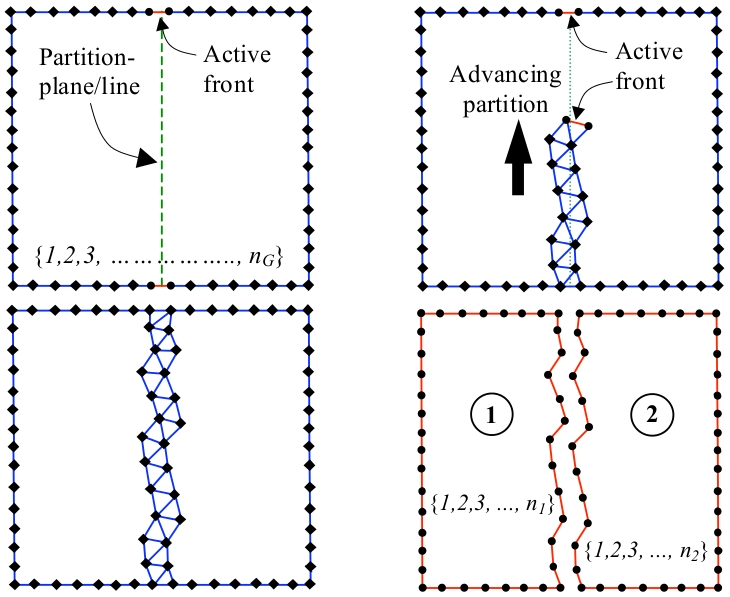
\includegraphics[width=0.8\textwidth]{imagem1}
     \caption{Os principais passos da técnica de \cite{bib:Pirzadeh09}.}
     \label{fig:imagem1}
 \end{figure}
 
 Como vantagens dessa técnica podemos citar que a utilização de avanço de camadas entre as partições faz com que a malha gerada seja praticamente idêntica a uma malha gerada sequencialmente, ou seja, não são gerados padrões entre as partições do domínio. Outra vantagem é que não é necessário nenhum pré-processamento para definir ou construir as partições.

\section{Decomposição baseada na distância/volume/centro de massa}
 
Em \cite{bib:Ivanov06}, foi desenvolvido um algoritmo baseado em Delaunay em que o posicionamento do plano de corte é definido pelo centro de massa e pela matriz de inércia. O plano de corte é um plano perpendicular a um eixo que segue uma das três definições:

\begin{itemize}
  \item Planos criados são equidistantes;

  \item Volume entre os planos são iguais;

  \item Passa pelo centro de massa.
\end{itemize}

A escolha do critério utilizado para criar os subdomínios vai depender da geometria da entrada. Dependendo da entrada, um critério pode ser melhor que outro, isso depende do conhecimento do usuário. Na Figura~\ref{fig:imagem2}, as três formas de decomposição são apresentadas.

Após ter o plano de corte definido, é feita uma suavização da seção de corte e a sua triangulação para, posteriormente, serem geradas as malhas nos subdomínios. Um problema bem visível nesse método é que para se ter um bom plano de corte é preciso ter um modelo com uma geometria bem comportada, sem forma côncava, alongada ou afinada.

 \begin{figure}[htbp]
     \centering
     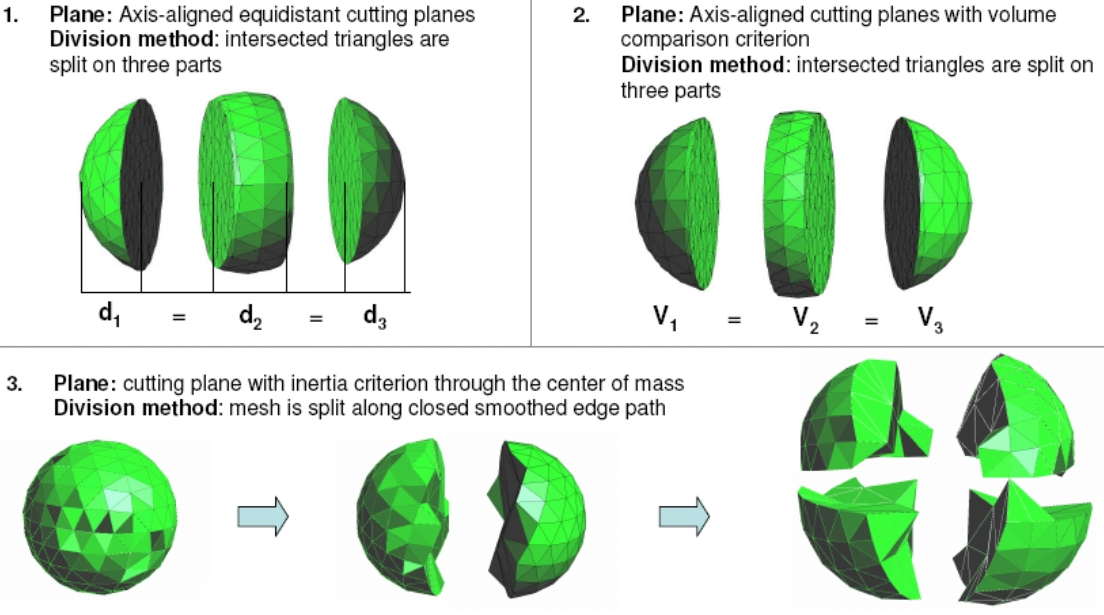
\includegraphics[width=0.9\textwidth]{imagem2}
     \caption{As 3 formas de particionar. 1 - planos equidistantes. 2 - volume dos subdomínios iguais. 3 - centro de massa \cite{bib:Ivanov06}.}
     \label{fig:imagem2}
 \end{figure}

Uma solução parecida é a apresentada em \cite{bib:Lammer00}, em que o plano de corte é traçado da mesma maneira, porém em duas dimensões, ou seja, um eixo de corte. Este eixo é usado para dividir o domínio recursivamente. A partir do eixo, uma aresta é formada, e os valores nos seus pontos extremos são interpolados dos valores dados como entrada. Quando o número de subdomínios for igual ao número de processadores, uma malha de Delaunay é gerada em cada interior.

\section{Decomposição baseada em \textit{octree}/\textit{quadtree}}

Em \cite{bib:deCougny99}, a entrada do algoritmo é o contorno de um objeto. Cada processador terá parte de uma \textit{octree} distribuída, que define planos de corte do domínio. A malha das células internas é gerada concorrentemente com \textit{templates}. A região entre o contorno e as células internas é preenchida por uma técnica de avanço de fronteira, onde são gerados os elementos internos a uma região delimitada pelos planos de corte. Por último é feita a conexão das malhas dos dois lados de cada plano e de suas intersecções.

Na técnica de \cite{bib:Lohner01}, é gerada uma \textit{octree} grosseira com relação ao contorno dado como entrada. Então, as células que contêm a parte da fronteira que gerará os menores elementos são identificadas. Assim, partes da malha, correspondentes a cada célula, são geradas simultaneamente por avanço de fronteira, de maneira que cada parte da malha gerada não possa cruzar as extremidades da célula que a contém. Então, cada octante sofre um pequeno deslocamento na diagonal com o intuito de gerar mais elementos. Esse deslocamento elimina quase todas as faces entre duas ou mais células e diminui o tamanho da fronteira para o próximo passo. Assim, a nova fronteira é encontrada, uma nova \textit{octree} é construída para ela, e o procedimento é repetido, até que não seja mais possível gerar malha.

Em \cite{bib:Larwood03}, é apresentada uma técnica de decomposição de domínio que tem como entrada uma triangulação de borda. Para saber quais subdomínios devem ser divididos, o autor usa um critério baseado na quantidade de faces por subdomínio. A decomposição é feita recursivamente usando uma \textit{octree} caso seja tridimensional ou uma \textit{quadtree} caso seja bidimensional, verificando sempre se o número de faces de um subdomínio é menor do que o limite estipulado, e, enquanto a verificação for falsa, a decomposição ocorre. A quantidade máxima de subdivisões está limitada por uma constante maior que o número de processadores disponíveis. Isso evita a criação excessiva de partições e permite que um processador possa receber mais de uma tarefa ao longo da execução.

Para evitar a criação de elementos ruins, é feita uma verificação no corte baseada no ângulo do vetor normal do plano de corte com a normal dos triângulos, de forma que o plano de corte não possa passar por triângulos com ângulo menor do que uma tolerância. Caso essa verificação falhe, a \textit{octree} (\textit{quadtree}, em 2D) sofre um deslocamento em um dos eixos. A Figura~\ref{fig:imagem3} mostra um exemplo onde alguns planos de corte falham nos testes.

 \begin{figure}[htbp]
     \centering
     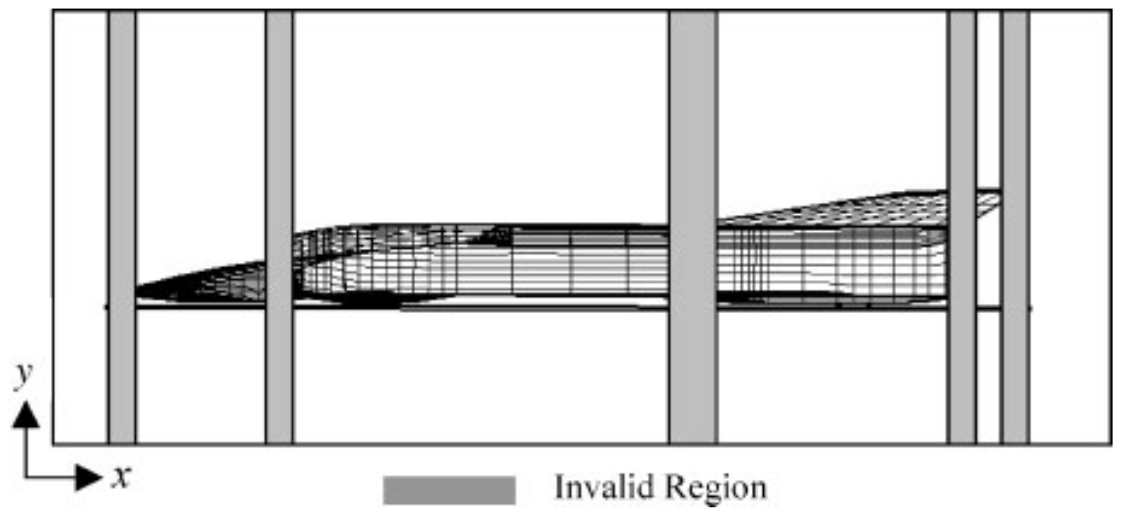
\includegraphics[width=0.9\textwidth]{imagem3}
     \caption{Regiões de corte inválidas em cinza \cite{bib:Larwood03}.}
     \label{fig:imagem3}
 \end{figure}

\section{Decomposição baseada no eixo mediano}

O eixo mediano é uma maneira de descrever a forma de um objeto, e é utilizado para garantir uma decomposição de domínio com separadores que formam bons ângulos com as bordas.

Em \cite{bib:Leonidas06}, é apresentada uma técnica bidimensional que utiliza a triangulação de Delaunay por divisão e conquista para um conjunto de pontos dados como entrada. Primeiramente, é feita uma triangulação utilizando apenas os pontos da borda, que é utilizada para a geração de um grafo ponderado, onde o peso de uma aresta é igual ao raio da circunferência circunscrita do triângulo que a contém. Em seguida é feita uma contração desse grafo. 

 \begin{figure}[htbp]
     \centering
     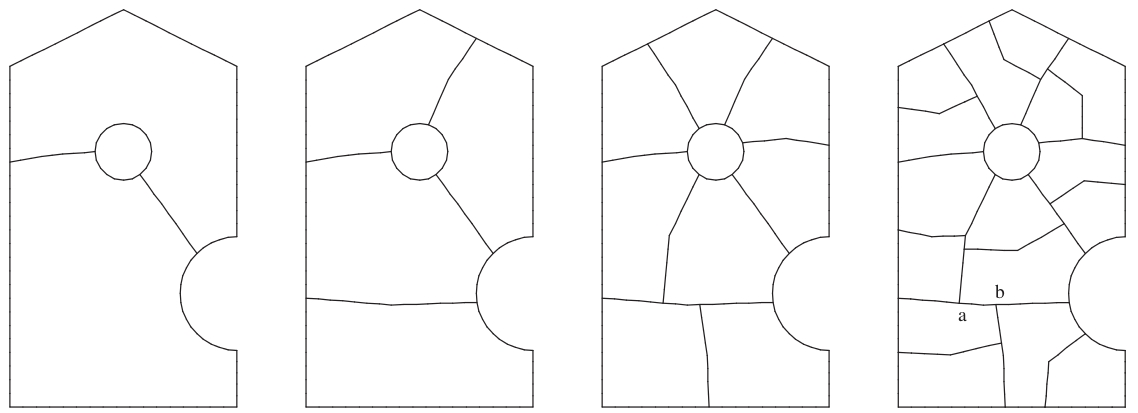
\includegraphics[width=0.9\textwidth]{imagem4}
     \caption{Partições em 2, 4, 8 e 16. \cite{bib:Leonidas06}.}
     \label{fig:imagem4}
 \end{figure}

Através do grafo formado, os planos de corte são posicionados e os subdomínios formados. A Figura~\ref{fig:imagem4} mostra o resultado de decomposições para quantidades diferentes de subdomínios. Após isso a geração da malha interna poderá ser realizada.

\section{Decomposição baseada em \textit{bounding Box}}

Em \cite{bib:Glut08}, é apresentada uma técnica para malhas tridimensionais. Essa é uma abordagem baseada na decomposição geométrica onde a entrada é uma malha de superfície. Aqui são apresentadas duas técnicas baseadas na \textit{bounding box} gerada a partir da entrada.

A seleção do separador do domínio deve garantir um custo de corte baixo, ou seja, encontrar e posicionar o plano de corte não pode ter um custo computacional alto. Além disso, deve garantir um bom balanceamento de carga e minimizar os elementos conectados por múltiplos subdomínios.

A primeira técnica é baseada na malha de superfície. Para o plano de corte ser criado, é preciso a localização do contorno da malha de superfície e do separador. O contorno é então projetado no separador usando uma função 2D de controle espacial baseada no tamanho das arestas (Figura~\ref{fig:imagem5}).

 \begin{figure}[htbp]
     \centering
     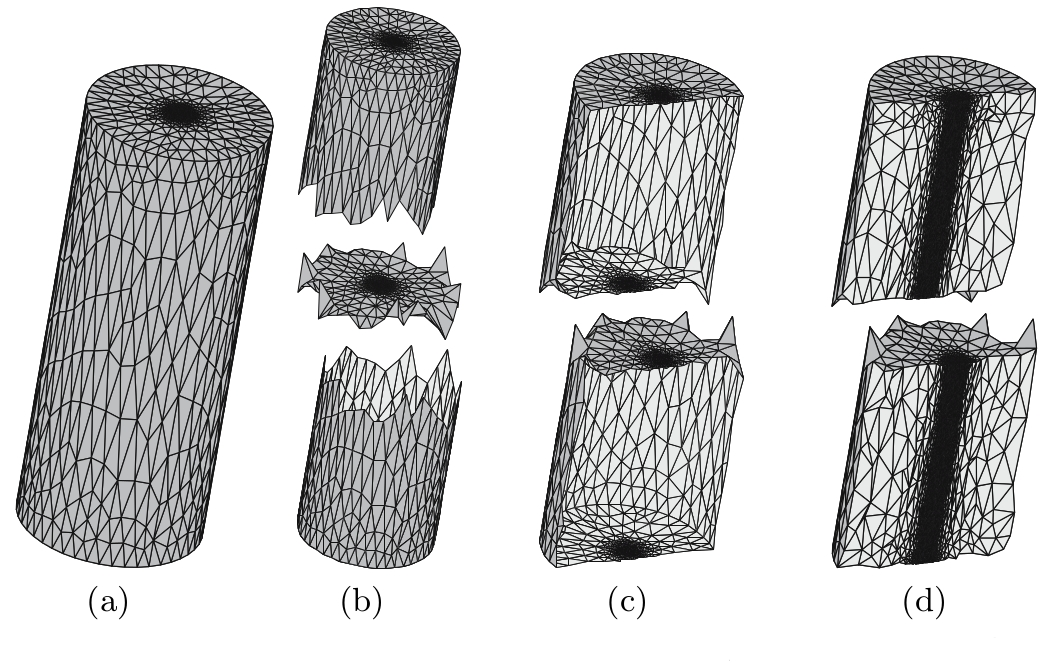
\includegraphics[width=0.9\textwidth]{imagem5}
     \caption{Passos da técnica baseada na malha de superfície. (a) malha de superfície; (b) corte; (c) seção transversal; (d) malha final. \cite{bib:Glut08}.}
     \label{fig:imagem5}
 \end{figure}

A segunda técnica se baseia numa malha volumétrica grosseira. Primeiramente, é feita a geração de uma malha 3D grosseira utilizando alguma função de controle espacial. O posicionamento do plano de corte é feito parecido com a técnica anterior, porém utilizando a malha volumétrica como função espacial (Figura~\ref{fig:imagem6}).

 \begin{figure}[htbp]
     \centering
     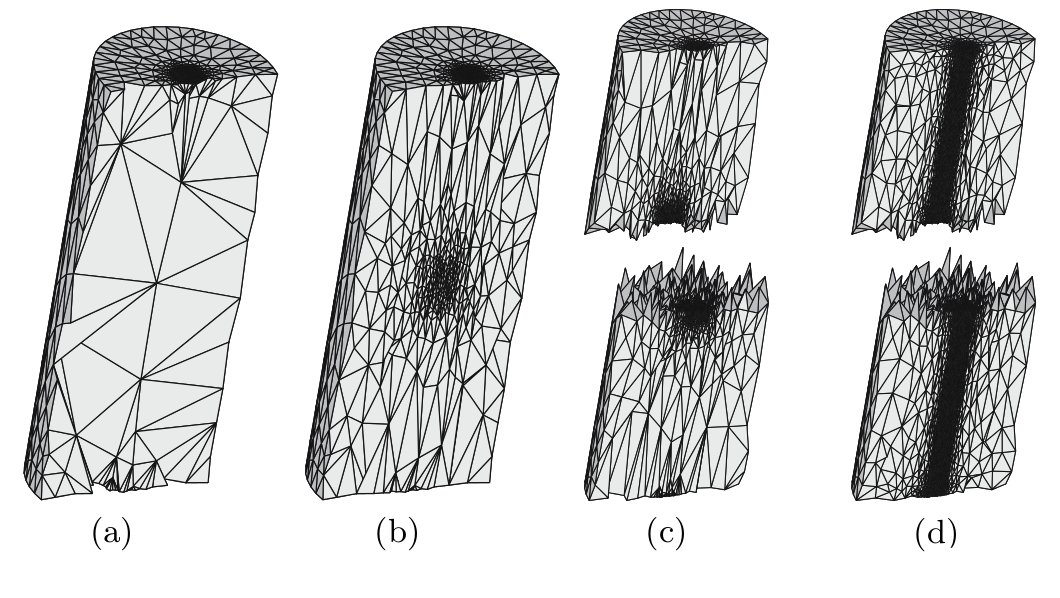
\includegraphics[width=0.9\textwidth]{imagem6}
     \caption{Passos da técnica baseada na malha volumétrica grosseira. (a) malha volumétrica grosseira; (b) refinamento da seção transversal; (c) seção transversal; (d) malha final. \cite{bib:Glut08}.}
     \label{fig:imagem6}
 \end{figure}

Essa técnica depende muito da geometria da entrada já que são utilizadas informações da \textit{bounding box} da entrada. Isso afeta diretamente a criação dos planos de corte e por consequência a malha gerada ao final.

	% Capítulo 2: Complexidade Descritiva
\pagestyle{empty}
\cleardoublepage
\pagestyle{fancy}

\chapter{Geração de Malhas}\label{cap3}

Nesse capítulo, serão apresentadas as técnicas de geração de malhas bidimensionais mais conhecidas atualmente. Existem diversos algoritmos para geração de malhas, porém todos eles podem ser enquadrados em três categorias que iremmos descrever a seguir:

\begin{itemize}
  \item Avanço de fronteira: a malha deve ser gerada a partir da borda da região;

  \item Delaunay: procura-se maximizar o menor ângulo dos triângulos gerados para um dado conjunto de pontos;

  \item Arbitrária: para todos os outros tipos de malhas;
\end{itemize}

\section{Avanço de fronteira}

Este é um dos métodos mais populares de geração de malhas e consiste em criar os elementos no interior do domínio progressivamente a partir de um contorno especificando da região a ser preenchida (fig.~\ref{fig:imagem7}a). Este contorno é chamado de fronteira inicial ou borda, os elementos são gerados a partir dessa fronteira dada como entrada. Uma fronteira bidimensional é formada por um conjunto de arestas.

À medida em que o algoritmo progride, a fronteira avança em direção ao interior, sempre removendo ou adicionando elementos de fronteira até que todo o domínio seja preenchido. O algoritmo chega ao fim quando não há mais fronteira, ou seja, o domínio foi totalmente triangularizado. 

Pode ocorrer do algoritmo não conseguir mais gerar elementos para uma determinada fronteira, isso indica que o algoritmo falhou. O caso de falha ocorre quando todos os possíveis elementos a serem criados se sobrepõe um elemento já existente. Por a importancia de verificar se um elemento criado não sobrepõe um elemento já existente. Os casos de falha geralmente acontecem em modelos tridimensionais.

Para gerar os novos triângulo no interior do domínio é necessário criar novo pontos que não pertencem à entrada, em geral é utilizados os pontos de Steiner para isso.

Enquanto houver arestas na fronteira um algoritmo nessa categoria irá proceded da seguinte forma no caso 2D (fig.~\ref{fig:imagem7}):
 
 \begin{enumerate}
\item{ Remova uma aresta da fronteira, a aresta base (fig.~\ref{fig:imagem7}b)}
\item{ Encontre um ponto ideal para a formação de um novo triângulo com a aresta base (fig.~\ref{fig:imagem7}c),}
\item{ Crie uma região de busca em torno desse ponto ideal (fig.~\ref{fig:imagem7}d),}
\item{ Selecione o ponto dentro dessa região de busca cujo triângulo (entre esse ponto e a aresta base) seja válido e seja o de melhor qualidade,}
\item{ Forme o novo triângulo com o ponto selecionado e adicione-o à malha (fig.~\ref{fig:imagem7}e),}
\item{ Atualize a fronteira, inserindo as arestas que foram criadas, e removendo as arestas que já existiam,}
\item{ Se existir aresta na fronteira, volte para o passo 1.}
\end{enumerate}

 \begin{figure}[htbp]
     \centering
     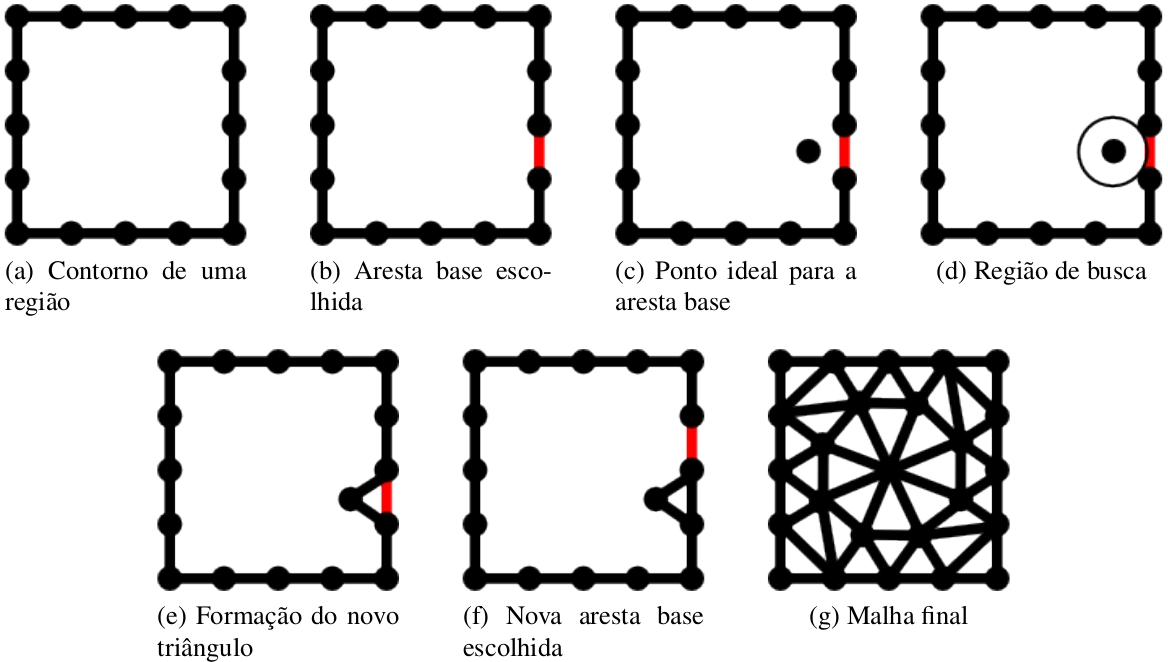
\includegraphics[width=1\textwidth]{imagem7}
     \caption{Avanço de fronteira. \cite{bib:Freitas10}} 
     \label{fig:imagem7}
 \end{figure}

 Pelo fato da fronteira ser sempre respeitada, os algoritmos de avanço de fronteira têm facilidade em tratar regiões descontínuas, ou por conterem buracos, ou por serem regiões separadas. Como os elementos mais próximos da borda são gerados primeiro, eles irão ter em geral uma boa qualidade. A boa qualidade da malha gerada provem estabilidade e precisão na aplicação de métodos numéricos (como os métodos dos elementos finitos).

Porém, nem sempre todos os elementos gerados terão boa qualidade. Ao contrário dos elementos mais próximos da borda, os elementos mais internos à malha nem sempre teão boa qualidade devido à região torna-se menor a medida que a fronteira avança. Geralmente uma técnica de suavização ou otimização é aplicada na malha resultante do algoritmo para tratar esses casos.
	% Capítulo 3: Classes de Complexidade Probabilisticas
\pagestyle{empty}
\cleardoublepage
\pagestyle{fancy}
\chapter{Lógicas Probabilísticas}\label{cap4}

Várias aplicações da Ciência da Computação necessitam da habilidade de raciocinar com informções incertas. Por exemplo, precisamos analisar programas probabilísticos, raciocinar sobre suposições probabilísticas da entrada e, em sistemas especialistas, várias regras obtidas dos especialistas são incertas. Já que as lógicas clássicas são úteis apenas nos casos onde temos certeza do conhecimento, várias propostas de extensão de lógicas para lidar com incertezas foram feitas. Algumas dessas propostas utilizaram a teoria da probabilidade para estender a lógica clássica e obter lógicas para poder lidar com informações incertas. Algumas dessas abordagens podem ser encontradas em \cite{fagin88, nilsson93, nilsson86, Halpern90ananalysis, Abadi1989, Fagin1994}. Abordagens mais recentes que utilizam apenas fragmentos da lógica de primeira ordem pode ser encontrados em \cite{Lukasiewicz08, LutzSchoder10, DurigStuder05, Cozman08LPP, TaoWHL07}.
Neste trabalho vamos mostrar duas abordagens diferentes. Elas foram introduzidas em \cite{Bacchus1991, Bacchus90} e foram analisadas em \cite{Halpern90ananalysis, Abadi1989}. Essas lógicas diferem basicamente no modo como a probabilidade é inserida.
Na primeira a probabilidade é inserida no domínio da estrutura, ou seja, cada elemento do domínio tem uma probabilidade associada. Na segunda temos um conjunto de estados ou mundos possíveis e cada um tem uma probabilidade.

\section{Probabilidade no Domínio}
Aqui temos a linguagem usual da Lógica de Primeira Ordem adicionada de uma função $w$ sobre as fórmulas. Seja $\phi$ uma fórmula na lógica, a fórmula $w_x(\phi) \ge \frac{1}{2}$ significa que a probabilidade de um $x$ aleatório satisfazer $\phi$ é maior ou igual a $\frac{1}{2}$. Para entender a intuição dessa fórmula suponha $\phi = Son(x, y)$. $w_x(\phi)$ representa a probabilidade de um elemento aleatório $x$ do domínio ser filho de $y$. A fórmula $w_y(\phi)$ descreve a probabilidade de $x$ ser filho de um $y$ aleatório. Também podemos ter a fórmula $w_{\tuple{x, y}}(\phi)$ que representa a probabilidade de um par de indivíduos $(x, y)$ terem  propriedade de $x$ ser filho de $y$.

Para formalizar essa intuição da função $w$ precisamos usar uma linguagem poli-sortida. Vamos usar uma estrutura poli-sortida $\mathcal{P} = \langle A, \mathbb{R},  R_{1}^{A}, ..., R_{r}^{A}, c_1^{A}, ..., c_s^{A}$, $ >^{\mathbb{R}}, +^{\mathbb{R}}, *^{\mathbb{R}}, 0^{\mathbb{R}}, 1^{\mathbb{R}}, \mu \rangle$, onde o domínio $A$ e as relações sobre e constantes sobre $A$ fazem parte do domínio que queremos representar. Já o segundo domínio $\mathbb{R}$ e as relações, funções e constantes sobre ele representam as probabilidades. O $\mu$ é uma função de probabilidade discreta sobre $A$, ou seja, $\mu : A \to [0, 1]$ tal que $\sum_{a \in A}\mu(a) = 1$. Para qualquer subconjunto $S \subseteq A$ fazemos $\mu(S) = \sum_{s \in S}\mu(s)$. Agora podemos definir a função $\mu^n$ para atribuir uma probabilidade para $n$ elementos do domínio, ou seja, $\mu^n(a_1, ... a_n) = \mu(a_1)*...*\mu(a_n)$.

Na linguagem, além do usual da linguagem de primeira ordem, temos dois tipos de variáveis: $VAR_A = \{x, y, z, ...\}$ e $VAR_{\mathbb{R}} = \{r_0, r_1, ... \}$, o primeiro conjunto de variáveis correspondem ao domínio $A$ e o segundo conjunto para os reais. Os termos do domínio são formados da maneira usual. O termos dos reais são variáveis em $VAR_{\mathbb{R}}$, as constantes 0, 1 e termos de probabilidade da forma $w_{x_1,...,x_n}(\phi)$. Além disso esses termos dos reais são fechados sobre as funções restritas aos reais. 

As fórmulas convencionais são formadas da maneira padrão restritas aos termos do domínio. Se $t_1$ e $t_2$ são dois termos dos reais então $t_1 > t_2$ e $t_1 = t_2$ também são fórmulas. 

A noção de interpretação e satisfação é feita como o usual. Uma interpretação é uma estrutura poli-sortida e uma função de assinalamento $\beta$ que mapeia elementos de $VAR_A$ em $A$ e elementos de $VAR_{\mathbb{R}}$ em $\mathbb{R}$.
A interpretação de termos do domínio também é feita da forma usual mas com a restrição de mapeamento em $A$. Para o caso dos termos dos reais, a diferença está nas probabilidades das fórmulas que é feita da seguinte forma:
\begin{center}
$(\mathcal{P}, \beta)(w_{\tuple{x_1,..., x_n}}(\phi)) = \mu^n(\{a_1, ..., a_n  \} : (\mathcal{P}, \beta[a_1/x_1, ..., a_n/x_n]) \models \phi)$. 
\end{center} 

A satisfação é feita de forma semelhante à da lógica de primeira ordem clássica.

\section{Probabilidade nos Mundos Possíveis}
Aqui, no lugar de inserirmos na linguagem $w_{\tuple{x_1,..., x_n}}(\phi)$ vamos colocar apenas $w(\phi)$ significando a probabilidade de $\phi$. Isso acontece pois não existe mais uma probabilidade associada aos elementos do domínio $x_1,..., x_n$. 

Agora temos uma distribuição de probabilidade em um conjunto de mundos possíveis onde em alguns desses mundos temos que a fórmula $\phi$ é verdade. A probabilidade da fórmula vai ser exatamente a probabilidade dos estados onde a fórmula é verdadeira.

Para formalizar, agora a estrutura é igual a anterior adicionada de um conjunto de estados, ou seja, $\mathcal{P}$ $= \langle A, S, \mathbb{R},  R_{1}^{A,s_1}, ..., R_{r}^{A,s_1}$, $ ..., R_{1}^{A,s_n}, ..., R_{r}^{A,s_n}$ $, c_1^{A, s_1}, ..., c_s^{A, s_1}, ..., c_1^{A, s_n}, ..., c_s^{A, s_n}$ $, >^{\mathbb{R}}, +^{\mathbb{R}}, *^{\mathbb{R}}, 0^{\mathbb{R}}, 1^{\mathbb{R}}, \mu \rangle$, onde $A$ é o domínio, $S$ é o conjunto de estados ou mundos possíveis, para cada estado $s \in S$ temos relações $R_i$ de aridade $a_i$ e constantes $c_i$. $\mu$ é uma função de probabilidade discreta em $S$. 

Uma interpretação agora é uma tripla $(\mathcal{P}, s, \beta)$, ou seja, agora é necessário saber qual estado está sendo avaliado. A interpretação dos termos é feita da maneira anterior mas agora cada estado pode levar à uma interepretação diferente dos termos. A interpretação da probabilidade de uma fórmula $w(\phi)$ é feita da seguinte maneira: 
\begin{center}
$(\mathcal{P}, s, \beta)(w(\phi)) = \mu(e \in S : (\mathcal{P}, e, \beta) \models \phi)$
\end{center}

A noção de satisfação é feita como o usual mas levando em conta o estado. Como exemplo vamos mostrar o caso em que uma interpretação $\mathcal{I} = (\mathcal{P}, s, \beta)$ satisfaz a fórmula atômica:
\begin{center}
$\mathcal{I} \models P(t_1, ..., t_n)$ se e somente se $\tuple{\mathcal{I}(t_1), ..., \mathcal{I}(t_n)} \in P^{A, s}$
\end{center}

Agora que mostramos essas duas lógicas probabilísticas, no próximo capítulo vamos comentar o que pretendemos fazer com elas e com as definições e resultados dos capítulos anteriores.	% Capítulo 4: Logicas Probabilisticas
\pagestyle{empty}
\cleardoublepage
\pagestyle{fancy}
\chapter{Direções Futuras}\label{cap4}

Foi feito um estudo nessa área de geração de malhas voltado para a subdivisão de domínios bidimensionais. Já foi dado início ao desenvolvimento de uma técnica de geração de malha baseada num particionamento utilizando \textit{quadtree}.

Este trabalho que estou propondo pode ser dividido basicamente em duas etapas. A primeira consiste em receber a entrada e dividi-la em pedaços que possam ser tratadas como novos domínios. Todos esses pedaços por sua vez possuem a quantidade de carga aproximadamente equivalentes.

Existem vários pesquisadores estudando novas formas de subdividir domínios para geração de malhas tanto tridimensionais como bidimensionais. A técnica proposta utiliza uma \textit{quadtree} para estimar a carga de cada subdomínio que for gerado para se obter um bom balanceamento de carga entre os processadores.

A segunda etapa será a geração da malha em cada um dos novos domínios. Qualquer algoritmo de triangulação dado uma borda como entrada pode ser utilizado, inclusive podem ser empregado algoritmos diferentes nos subdomínios. Além da triangulação, tem que ser feita a junção das diversas malhas geradas em uma só.

Para esse trabalho estou propondo uma técnica de geração de malha por avanço de fronteira por particionamento do domínio em paralelo. O foco da técnica é a subdivisão dos domínios e não a geração da malha. O algoritmo de avanço de fronteira que estou utilizando para gerar malha está em \cite{bib:Miranda99} e \cite{bib:Cavalcante-Neto01}.

\section{Cronograma}
Nesta seção apresento o cronograma de estudo e trabalho para conclusão da dissertação de mestrado.

 \begin{figure}[htbp]
     \begin{center}
     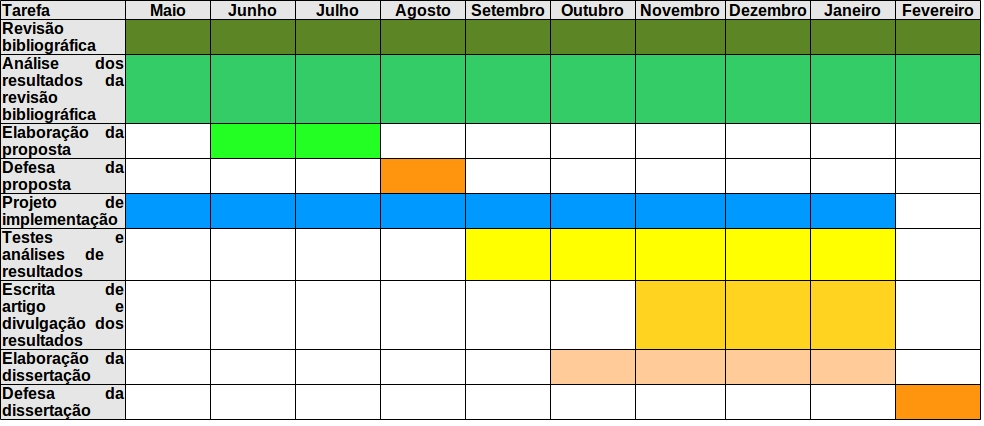
\includegraphics[width=1.1\textwidth]{tabela}
     \label{fig:tabela}
     \end{center}
 \end{figure}	% Capítulo Final: Considerações Finais

% Formato da bibliografia
%\bibliographystyle{apalike}
\bibliographystyle{plain}
% Arquivo .bib
\bibliography{mestre}

% Apêndice(s)
%\include{apendice}

% Fim do texto
\end{document}
